\newpage

\section{Theoretische Grundlagen}
\label{sec:theorie}

\subsection{Business Intelligence im Energiesektor}
\label{subsec:bi-energie}

Müller und Lenz beschreiben \textbf{Business Intelligence (BI)} augenzwinkernd als
\begin{quote}
    „50\,\% BWL + 25\,\% Statistik + 25\,\% Data Warehouse.“
\end{quote}
BI stellt damit die Verbindung zwischen Daten und deren gezielter Auswertung mit statistischen Methoden zur Erkenntnisgewinnung dar (vgl.\ \citeauthor{mueller2013} \citeyear{mueller2013}, S.~3f).

Der weltweite Energieverbrauch hat sich seit 1990 nahezu verdoppelt (vgl. \citeauthor{enerdata2025} \citeyear{enerdata2025}). Je nach Jahreszeit, Wirtschaftslage und unter dem Einfluss äußerer Faktoren ist die Energienachfrage äußerst volatil. Sowohl die Politik als auch Energieversorgungsunternehmen haben daher großes Interesse, den zukünftigen Energieverbrauch mithilfe geeigneter Analysetechniken möglichst realitätsnah prognostizieren zu können, um Produktion und Investitionen entsprechend abstimmen zu können. Verlässliche Analysen können sich dabei zu einem entscheidenden Erfolgsfaktor entwickeln. Moderne BI-Systeme ermöglichen es, historische Verbrauchsdaten mit externen Einflussgrößen – etwa Witterung, Konjunkturindikatoren oder geopolitischen Ereignissen – zu verknüpfen, um daraus verwertbare Erkenntnisse zu generieren.

Im Zentrum dieser Arbeit steht der Einsatz von Zeitreihenanalysemodellen zur Vorhersage von Energieverbrauchsmustern in den Vereinigten Staaten. Ziel ist es, durch den Vergleich verschiedener Prognoseverfahren – insbesondere ARIMA- und Holt-Winters-Modelle – zu untersuchen, inwiefern diese zur energiepolitischen Entscheidungsfindung beitragen können, insbesondere im Hinblick auf krisenhafte Schocks wie die COVID-19-Pandemie oder den russischen Angriffskrieg gegen die Ukraine.


\subsection{Grundlagen der Zeitreihenanalyse}
\label{subsec:ts-grundlagen}

Eine Zeitreihe ist eine Menge von periodischen Beobachtungen (Phänomene), denen jeweils ein Wert zugeordnet ist - beispielsweise das Brutto-Inlandsprodukt eines Landes pro Jahr. Die beobachtete Menge $X_t=x_0, x_1,...,x_t$ enthält die Zeitpunkte der Beobachtung (meist periodisch) $t$ sowie den zugeordneten Wert $x_t$ (vgl. \citeauthor{leiner1998} \citeyear{leiner1998}, S.~2f).
Eine Zeitreihe $X_t$ kann nach \cite{leiner1998} in mehrere Komponenten unterteilt werden.
\begin{itemize}
    \item Der \textbf{Trend $G_t$} zeigt die Richtung, bzw. Tendenz der beobachteten Werte über einen Zeitraum an (auf-, absteigend oder konstant)
    \item Die \textbf{Konjunkturkomponente $S_t$} zeigt Schwankungen in den Beobachtungen über mehrere Monate bis Jahre
    \item Die \textbf{Saisonkomponente $S_t$} enthält systematische Schwankungen (Muster), die über mehrere Perioden hinweg wiederholt auftreten (z.B. vermehrte Verkäufe von Eiscreme im Sommer)
    \item Die \textbf{irreguläre Komponente $U_t$} steht für den Einfluss von unsystematischen Störfaktoren, die nicht von anderen Komponenten aufgefangen werden können
\end{itemize}

Komponenten können \textbf{additiv:}
\begin{equation}
    X_t=G_t+K_t+S_t+U_t
\end{equation}
oder \textbf{multiplikativ:}
\begin{equation}
    X_t=G_t\cdot K_t \cdot S_t \cdot U_t
\end{equation}
zusammengefügt werden (vgl. \citeauthor{leiner1998} \citeyear{leiner1998}, S.~7).

Die Vorhersage basiert in der Regel auf der Annahme, dass sich vergangene Strukturen – zumindest kurzfristig – fortsetzen lassen. Die Analyse des Trendverlaufs erfolgt i.d.R. deterministisch, beispielsweise über das Finden einer Gerade, die den Trendverlauf möglichst genau darstellt (Lineare Regression). Laut \citeauthor{leiner1998} (\citeyear{leiner1998}, S.~52) können rund 75\% einer Zeitreihe schon allein durch den Trend erklärt werden - die restlichen 25\% erst mit der Konjunktur- und Saisonkomponente sowie Zufallseinflüsse. Eine Analyse dieser Komponenten erfodert komplexere mathematische oder statistische Modelle, wie beispielsweise das exponential smoothing, welches im Anschluss kurz erläutert wird.

\textbf{Kurvenglättung}
\begin{quotation}
Kurvenglättung (auch \textit{exponential smoothing}) dient der kurzfristigen Prognose zukünftiger Werte in Zeitreihen. Bei der einfachsten Variante, dem \textit{Simple Exponential Smoothing (SES)}, wird der nächste Wert $\hat{y}_{t+1}$ basierend auf den bisherigen Beobachtungen $y_0, \dots, y_t$ geschätzt. Jede Beobachtung wird gewichtet mit dem \textbf{Smoothing-Parameter} $\alpha$, der im Intervall $0 \leq \alpha \leq 1$ liegt. Beim SES gewichtet $\alpha$ neuere Daten stärker als weiter zurück liegende, da diese meist relevanter für die nächste Periode sind. Die Gewichtung für jeden Wert, der weiter in der Vergangenheit liegt nimmt exponentiell ab - daher auch der Name. Je kleiner $\alpha$, desto weniger Einfluss hat der jeweilige Wert auf die Vorhersage von $\hat{y}_{t+1}$. Die Formel der exponentiellen Kurvenglättung einer Zeitreihe $X_t$ ist:
\begin{equation}
    \hat{y}_{t+1}=\alpha \cdot y_t+\alpha(1-\alpha)\cdot y_{t-1}+\alpha(1-\alpha)^2\cdot y_{t-2}+\alpha(1-\alpha)^3\cdot y_{t-3}\dots
\end{equation}
Die Vorhersage der weiteren Prognosewerte SES ist ein \textit{weighted average} der letzten Beobachtung $y_t$ und der letzten Vorhersage $\hat{y}_{t-1}$. \cite{hyndman2018}
\end{quotation}

Eine geeignete Auswahl des Modells ist je nach Anforderung an die Analyse ein wichtiger Erfolgsfaktor für die Genauigkeit späterer Prognosen. Das in dieser Arbeit verwendete \textbf{Holt-Winters} Verfahren zur Kurvenglättung sowie die \textbf{ARIMA} bzw. \textbf{SARIMA} Modelle werden im nächsten Abschnitt näher beschrieben.


\subsection{Prognosemodelle: Holt-Winters, ARIMA und SARIMA}
\label{subsec:prognosemodelle}
\subsubsection{Holt-Winters}
Das \textbf{Holt-Winters-Modell} erweitert die einfache exponentielle Glättung um den Einfluss von Trend- und Saisonkomponenten. Es existieren additive und multiplikative Varianten von Holt-Winters. Die \textit{additive Form} ist für gleichbleibende Saisonschwankungen geeignet, die \textit{multiplikative Form} ist besser geeignet für sich proportional zur Höhe der Beobachtung ändernden Schwankungen. Holt-Winters berechnet für jede Beobachtung drei Komponenten und summiert diese.
\begin{equation}
y_{t} = l_t + h \cdot b_t + s_{t+h-m}
\end{equation}
mit:
\begin{itemize}
    \item $l_t$: Level (Höhe des Wertes zum Zeitpunkt $t$), mit $l_t=\alpha(y_t-s_{t-m})+(1-\alpha)(l_{t-1}+b_{t-1})$
    \item $b_t$: Wert des Trends an $t$, mit $b_t=\beta (l_t-l_{t-1})+(1-\beta)b_{t-1}$
    \item $s_t$: saisonale Komponente an $t$, mit $s_t=\gamma(y_t-l_{t-1}-b_{t-1})+(1-\gamma)s_{t-m}$
    \item $h$: Anzahl vorausgesagter Perioden
    \item $M$: Periodenlänge der Saisonalität (z.B. $M = 12$ bei monatlichen Daten mit Jahres-Saisonalität)
    \item $\alpha, \beta and \gamma$: Smoothing Parameter der einzelnen Komponenten im Intervall $[0, 1]$
\end{itemize}
Da der Trend eine lineare Funktion und sich die saisonale Komponente zyklisch wiederholt, kann der Algorithmus für Prognosen fortgeführt werden. Der lineare Trend steigt oder sinkt weiterhin und die Saisonschwankungen werden zyklisch auf die Vorhersagen angewandt:

In der multiplikativen Form berechnet Holt-Winters ebenfalls die drei Komponenten, diese werden jedoch multipliziert, um sich größer werdenden Schwankungen anzugleichen:
\begin{equation}
\hat{y}_{t+k} = (L_t + h \cdot T_t) \cdot S_{t+h-m}
\end{equation}


\subsubsection{ARIMA}
\textbf{ARIMA} steht für \textbf{A}uto\textbf{R}egressive \textbf{I}ntegrated \textbf{M}oving \textbf{A}verage. Anders als beim deterministischen Holt-Winters Verfahren basiert ARIMA auf statistischen Methoden.
\textbf{Auto Regressive} bedeutet, dass vorherige Werte die aktuellen Werte linear beeinflussen. Die Formel der $\text{AR(p)}$ Komponente ist:
\begin{equation}
    y_t=\phi_1X_{t-1}+\phi_2X_{t-2}+\dots +\phi_pX_{t-p}+\epsilon_t
\end{equation}
Der Parameter $p$ gibt die Ordnung an, also wie viele vergangene Werte für die Berechnung des nächsten verwendet werden. $\phi_i$ ist die Gewichtung des jeweiligen vergangenen Werts und $\epsilon_t$ fügt der Komponente ein zufälliges Rauschen hinzu (Fehler) (vgl. \citeauthor{hyndman2018} \citeyear{hyndman2018}, Kap. 8.3).

Der \textbf{Moving Average} bezieht frühere Modell-Fehler mit ein. Starke Ausreißer durch Fehlannahmen des Modells werden mit Hilfe von Gewichtungen geglättet. Die Formel eines $\text{MA(q)}$ Modells der Ordnung $\text{q}$ ist wie folgend:
\begin{equation}
    y_t=c+\epsilon_t+\theta_1\epsilon_{t-1}+\theta_2\epsilon_{t-2}+\dots+\theta_q\epsilon_{t-q}
\end{equation}
$\theta_q$ gewichtet die jeweiligen vergangenen Modellfehler $\epsilon_i$ und $c$ ist der konstante Mittelwert der Zeitreihe (vgl. \citeauthor{hyndman2018} \citeyear{hyndman2018}, Kap. 8.4). 

Der \textbf{Integrated}-Teil setzt voraus, dass jede Zeitreihe \textit{stationäre} sein muss, damit ARIMA Modelle Prognosen tätigen können. \textit{Stationär} bedeutet, dass statistische Eigenschaften einer Zeitreihe nicht von der Zeit der Beobachtung abhängig sind. Auf lange Sicht haben stationäre Zeitreihen keine erkennbaren Muster - sie haben also keine Trend- oder Saisonkomponenten (vgl. \citeauthor{hyndman2018} \citeyear{hyndman2018}, Kap. 8.1). Mittels \textbf{Differenzierung} kann eine nicht-stationäre Zeitreihe in eine stationäre transformiert werden, um Varianz und Mittelwerte zu stabilisieren - so werden Trend und Saisonalität reduziert, was die Genauigkeit von ARIMA Modellen verbessert. Dies ist Voraussetzung, da bei der Autoregression vergangene Werte vergleichbar sein müssen. Die Linearkombinationen mit $\phi$ oder $\theta$ würden sonst bei nicht-stationären Zeitreihen zusätzlich abhängig von der Zeit sein. In diesen Fall sind ARIMA-Modelle nicht geeignet.

Um eine nicht-stationäre Zeitreihe in eine stationäre zu transformieren muss diese differenziert werden. Man spricht vom integrierten Teil $\text{I(d)}$ des Grades $d$, d.h. Die Zeitreihe musste $d$-mal differenziert werden, um stationär zu sein. Die erste Differenz zieht von jedem Wert aus den Beobachtungen $X_t$ den vorherigen Wert $X_{t-1}$ ab:
\begin{equation}
    Y_t^{'}=X_t-X_{t-1}
\end{equation}
Dies ist häufig schon ausreichend, um eine stationäre Zeitreihe zu erzeugen. Falls nicht, kann noch ein zweites mal differenziert werden. Diesmal:
\begin{equation}
    Y_t^{''}=Y_t-Y_{t-1}
\end{equation}
Um zu erkennen, ob ein Modell stationär ist, können visuelle Analysen, Funktionen wie \textbf{ACF} und \textbf{PACF} sowie der \textbf{ADF}-Test durchgeführt werden.
\textbf{Visuell:}\\
Trends oder Saisonalität können oft schon visuell erkannt werden
\textbf{(Partial) Auto-Correlation-Function (ACF/PACF):}\\
\\Die ACF-Funktion stellt die Korrelationen einer Zeitreihe mit verschobenen Versionen von sich selbst über verschiedene Zeitabschnitte (lags) dar. Ähnliche Werte innerhalb der lags bedeuten eine Korrelation dieser. Die PACF-Funktion isoliert die einzelnen lags und zeigt, wie stark sich jeder lag (also jeder Zeitabschnitt) individuell auf die Zeitreihe auswirkt, ohne den Einfluss der anderen lags (vgl. \citeauthor{kis2024} \citeyear{kis2024}).
\begin{figure}[htbp]
    \centering
    \begin{subfigure}[t]{0.48\textwidth}
        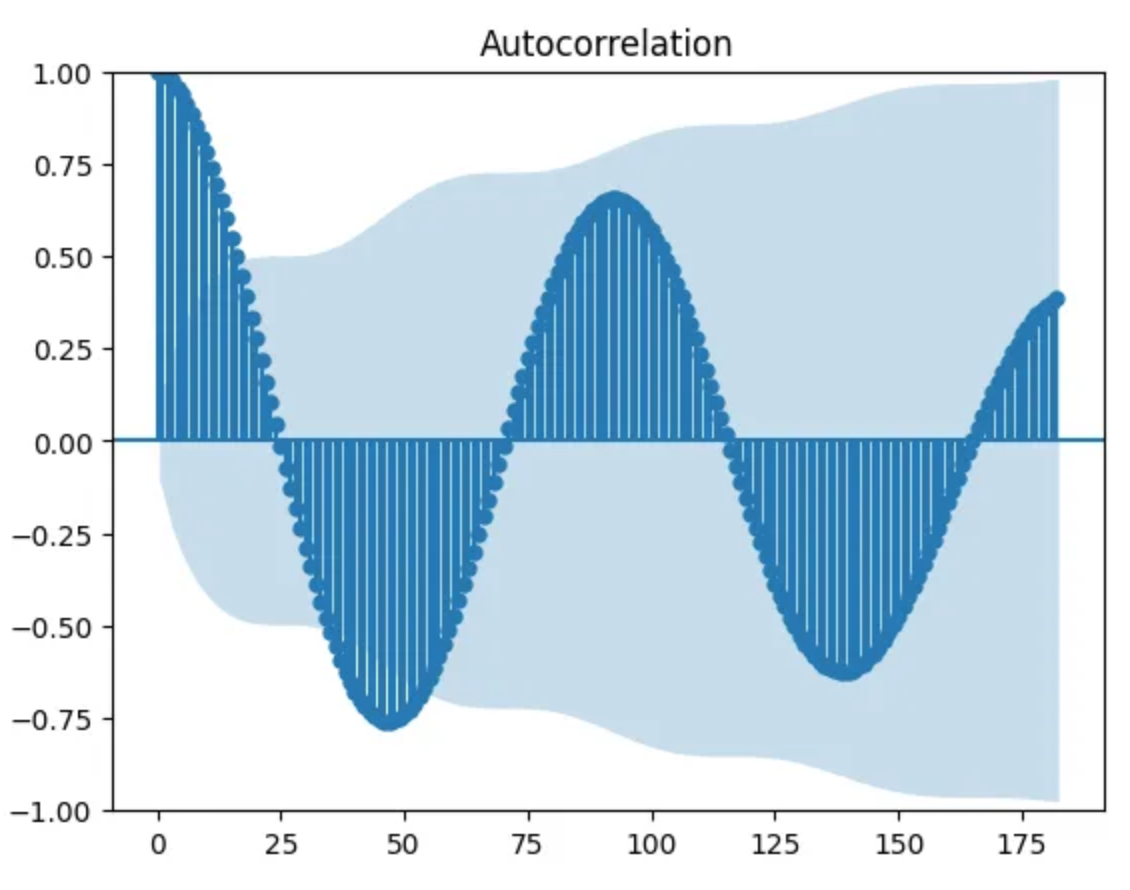
\includegraphics[width=\textwidth]{images/acs.png}
    \end{subfigure}
    \hfill
    \begin{subfigure}[t]{0.48\textwidth}
        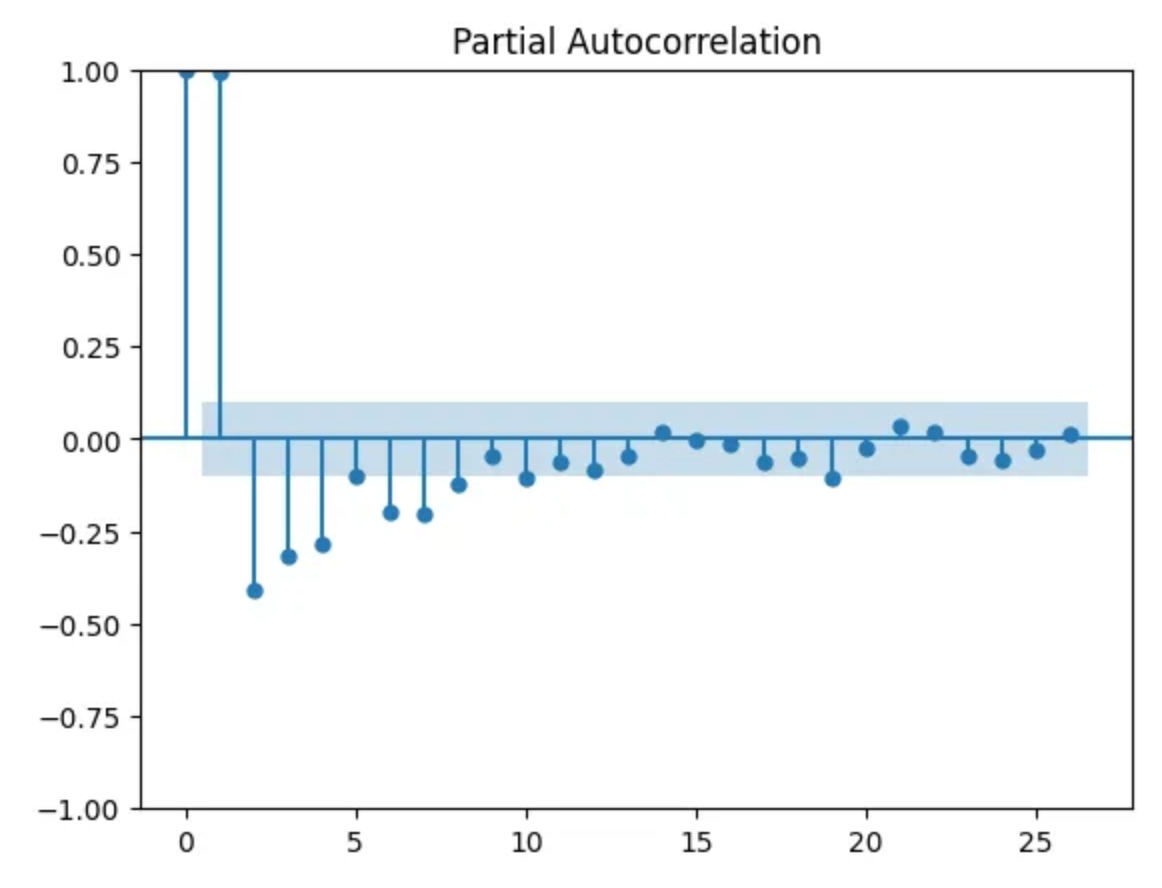
\includegraphics[width=\textwidth]{images/pacs.png}
    \end{subfigure}
    \caption{Autocorrelation (links) und Partial Autocorrelation (rechts)}
    \subcaption{\cite{kis2024}}
\end{figure}

Im ACF-Plot (links) erkennt man ein sinusoides Muster, was auf saisonale Zyklen hindeutet. Der PACF-Plot zeigt den sehr hohen Einfluss von lag 1, 2, 3, 4, 5, 7 und 8. Diese befinden sich ausserhalb des 95\% Konfidenzintervalls (blaues Band) und haben daher signifikanten Einfluss auf die gesamte Zeitreihe. \\
\\\textbf{Augmented Dickey-Fuller-Test (ADF):}\\
Statistisches Verfahren, das prüft, ob eine Zeitreihe eine Einheitswurzel enthält. Wenn eine Einheitswurzel-Charakteristik vorliegt wird ein Verschieben (lag) der Zeitreihe keine relevanten Informationen über die Prognose von $\hat{y_t}$ geben können. Wird eine Einheitswurzel gefunden liegt eine nicht-stationäre Zeitreihe vor. Wird im Gegenzug keine Einheitswurzel gefunden, kann von einer stationären Zeitreihe ausgegangen werden \cite{kwiatkowski1992}.\\
\\Das fertige ARIMA Modell wird also beschrieben mit den Parametern:
\begin{equation}
    ARIMA(p,d,q)
\end{equation}
Mit:
\begin{itemize}
    \item $p$: Ordnung der Autoregression (Wie viele vergangene Werte haben Einfluss auf den aktuellen Wert?)
    \item $q$: Ordnung des moving average (Wie viele vergangene Fehler werden haben Einfluss auf den aktuellen Wert?)
    \item $d$: Grad der Differenzierung bis die Zeitreihe stationär ist
\end{itemize}


\subsubsection{SARIMA}
ARIMA kann keine saisonalen Muster abbilden. Daher wird es zum \textbf{SARIMA-Modell} erweitert, indem es um die Parameter $(P, D, Q)_m$ ergänzt wird:
\begin{equation}
SARIMA(p,d,q)(P,D,Q)_m
\end{equation}
Hierbei beschreibt $m$ die saisonale Periodenlänge, z.\,B. $m=12$ für monatliche Daten mit jährlicher Saisonalität (vgl. \citeauthor{hyndman2018} \citeyear{hyndman2018}, Kap. 8.9).


\subsection{Bewertungsmetriken für Prognosegüte}
\label{subsec:metriken}

Zur Bewertung der Qualität von Vorhersagemodellen werden verschiedene statistische Fehlermaße verwendet. Die folgenden Metriken werden in dieser Arbeit zur Modellevaluation verwendet:

\paragraph{Mean Absolute Error (MAE):}
Der mittlere absolute Fehler gibt an, wie stark die Vorhersagewerte im Mittel von den tatsächlichen Werten abweichen \cite{vanderlei2020}:
\begin{equation}
\text{MAD} = \frac{1}{n} \sum_{t=1}^{n} |y_t - \hat{y}_t|
\end{equation}

\paragraph{Mean Absolute Percentage Error (MAPE):}
Die durchschnittliche prozentuale Abweichung des Fehlers von den jeweiligen tatsächlichen Werten \cite{vanderlei2020}.

\begin{equation}
\text{MAPE} = \frac{100}{n} \sum_{t=1}^{n} \left| \frac{y_t - \hat{y}_t}{y_t} \right|
\end{equation}

\paragraph{Root Mean Squared Error (RMSE):}
Die Wurzel des durchschnittlichen quadrierten Fehlers. Weniger anfällig für Ausreißer. Kann dank der Wurzel auch Modelle mit unterschiedlichen Skalen vergleichen.

\begin{equation}
\text{RMSE} = \sqrt{ \frac{1}{n} \sum_{t=1}^{n} (y_t - \hat{y}_t)^2 }
\end{equation}

Ein niedriger Wert dieser Metriken signalisiert eine hohe Prognosequalität. Die Auswahl geeigneter Metriken hängt dabei vom jeweiligen Anwendungsfall, der Skalierung der Daten und der Fehlertoleranz ab.
